\chapter{Results}
\label{results}

This chapter, discusses the performance of the AMM Scheduler. The objective of the discussed tests is the validation of the effectiveness of the proposed scheduling logics (Static, Static Hetero, and Dynamic) and to analyze how the workload is distributed among the available accelerators in a real-world heterogeneous environment.

All the experiments were conducted as already described in the Tool chapter (see Chap. \ref{tools}), on a modern high performance laptop, specifically the Lenovo Yoga Pro 9. 

The specific hardware and software used are listed below:
\begin{itemize} 
    \item CPU the Intel Core Ultra 9 185H.
    \item Intel Arc Graphics as the integrated GPU.
    \item Intel AI Boost NPU. 
    \item NVIDIA GeForce RTX 4060 Laptop (8GB VRAM). 
    \item RAM 32 GB DDR5. 
    \item OS Kubuntu 25.10 with the linux kernel 6.17. 
\end{itemize}

\section{Homogeneous Workloads}
The first set of tests are on homogeneous workloads, where the scheduler process batch of identical matrix multiplication tasks, we analyzed three different matrix sizes: 1024x1024, 2048x2048, and 4096x4096, all the data used are with 32 bit precision.

In this case, we compare the Static Partitioning logic against the Dynamic logic and for the baseline the CUDA only logic will be used. 

\clearpage

\subsection{Matrix: 1024x1024}
In this case, we are dealing with small matrices, where the biggest overhead is certainly the latency of moving data between memories. The results of the logic execution are presented below:

\begin{figure}[h!]
    \centering
    \includegraphics[scale=0.3]{images/results/compare_time_s1024.png} 
    \caption{Time Comparison 1024}
    \label{time1024}
\end{figure}

\begin{figure}[h!]
    \centering
    \includegraphics[scale=0.3]{images/results/compare_energy_s1024.png} 
    \caption{Energy Comparison 1024}
    \label{energy1024}
\end{figure}

As we can see from Figure \ref{time1024}, with these small tasks, the static logic and the dynamic logic perform almost in the same way, both clearly outperform the single CUDA card by using multiple accelerators in parallel. An average speedup of 2\% was observed for the static logic, and 2.10\% for the dynamic logic, compared to the CUDA logic. The graph in Figure \ref{energy1024} is very interesting, where we can clearly see how the two strategy manage to stay below the total consumption of the CUDA logic (for energy metrics, see Sec. \ref{implprofiler}). This is a very significant result because it shows how these different accelerators, even if they are not as fast as the CUDA card, can still be efficient; and if used in parallel, they lead to an increase in the total system efficiency. In this case, the metric efficiency was calculated as Tasks per Joule, and we obtained:

\begin{itemize}
    \item Cuda only: 2.62 Tasks/J
    \item Dynamic: 4.46 Tasks/J
    \item Static: 4.24 Tasks/J
\end{itemize}

Furthermore, to investigate the performance of the two logics, graphs were made to see how the tasks are distributed among the various accelerators, and how much time the accelerators actually work during the whole makespan.

\begin{figure}[h!]
    \centering
    \includegraphics[scale=0.3]{images/results/distrib_tasks_s1024.png} 
    \caption{Task Distribution 1024}
    \label{dist1024}
\end{figure}

\begin{figure}[h!]
    \centering
    \includegraphics[scale=0.3]{images/results/distrib_s1024.png} 
    \caption{Time Distribution 1024}
    \label{timedistr1024}
\end{figure}

Here we can see how the two logics fundamentally differ in their operation. The greedy nature of the dynamic logic tends to make the accelerators work more continuously in this case of small tasks, managing to "spread" the work better among the accelerators. As we can note from Figure \ref{dist1024}, it is clear that the static logic underestimated the performance of the non CUDA accelerators, and this led to a higher number of tasks on NVIDIA card, meanwhile, the dynamic logic managed, thanks to its greedy nature, to make the other accelerators work much more evenly, and this indeed led to a bit more faster times. In fact, as we can see from the graph in Figure \ref{timedistr1024}, the dynamic logic definitly make more use of the other accelerators over the CUDA card. This is due to the fact that they are slightly faster in this smaller tasks, having much less memory overhead.

\clearpage 

\subsection{Matrix: 2048x2048}
In this scenario, the workload increases significantly. The matrix size is large enough that the computational cost starts to increase over the data transfer overhead. The results of the logic execution are presented below:

\begin{figure}[h!] \centering \includegraphics[scale=0.3]{images/results/compare_time_s2048.png} \caption{Time Comparison 2048} \label{time2048} \end{figure}

\begin{figure}[h!] \centering \includegraphics[scale=0.3]{images/results/compare_energy_s2048.png} \caption{Energy Comparison Matrix 2048} \label{energy2048} \end{figure}

As shown in Figure \ref{time2048}, both strategies continue to outperform the single CUDA baseline, validating the benefit of parallel execution even in this kind of workload. However, a clear different appears between the two logics. The dynamic strategy achieves an average speedup of 2.21x (peaking at 2.71x), while the static strategy lags slightly behind with an average speedup of 1.90x. This indicates that the dynamic logic is 14\% faster on average for this specific workload. 

Regarding energy efficiency (Figure \ref{energy2048}) the heterogeneous execution significantly reduces the total energy consumption compared to the CUDA only approach, thanks to the reduction in total execution time. The dynamic strategy proves to be the most efficient, consuming only 218 J on average per batch, compared to 430 J for CUDA Only.

The efficiency metric show this gain: 
\begin{itemize} 
    \item \textbf{CUDA Only}: 0.66 Tasks/J 
    \item \textbf{Dynamic}: 1.14 Tasks/J 
    \item \textbf{Static}: 1.00 Tasks/J 
\end{itemize}

\begin{figure}[h!] \centering \includegraphics[scale=0.3]{images/results/distrib_tasks_s2048.png} \caption{Task Distribution: Matrix 2048x2048} \label{distrib2048} \end{figure}

\begin{figure}[h!] \centering \includegraphics[scale=0.3]{images/results/distrib_s2048.png} \caption{Time Distribution: Matrix 2048x2048} \label{timedistr2048} \end{figure}

Figure \ref{distrib2048} reveals again the cause of the performance difference. The static strategy assigns a large portion of tasks to the CUDA GPU and a smaller share to the other accelerators. While safe, this distribution appears to underutilize the other accellerators.

However, the dynamic strategy as already said, adapts in real time, so as seen in the Figure \ref{timedistr2048}, the dynamic logic keeps the CPU, the intel GPU and NPU work more evenly.

\subsection{Matrix: 4096x4096}
This scenario expose a heavy workload on the scheduler, the computational cost now should  dominate the ovehread of data transfer. The results of the logic execution are presented in Fig. \ref{time4096} and Fig. \ref{energy4096}:

\begin{figure}[h!] \centering \includegraphics[scale=0.3]{images/results/compare_time_s4096.png} \caption{Time Comparison 4096} \label{time4096} \end{figure}

\begin{figure}[h!] \centering \includegraphics[scale=0.3]{images/results/compare_energy_s4096.png} \caption{Energy Comparison 4096} \label{energy4096} \end{figure}

As shown in Figure \ref{time4096} both strategies still significantly outperform the single CUDA baseline. However, the static strategy show its superiority in this specific scenario, achieving an average speedup of 2.00x (peaking max at 2.90x) and the dynamic strategy follows with an average speedup of 1.78x (peaking at 2.67x). Ultimately, the static logic proves to be 12.5\% faster on average compared to the Dynamic one.

Regarding efficiency (Figure \ref{energy4096}), the results still shows that despite activating all available accelerators, the parallel execution reduces the total energy consumed, the CUDA-only execution consumes on average 568.70 J, while the heterogeneous strategies drop this to roughly 330-340 J.

\begin{itemize} \item \textbf{CUDA Only}: 0.11 Tasks/J \item \textbf{Dynamic}: 0.18 Tasks/J \item \textbf{Static}: 0.18 Tasks/J \end{itemize}

This represents a +61\% efficiency gain for the static strategy over the baseline: using the CPU and NPU alongside the GPU for heavy tasks actually saves energy because the entire system finishes the job much faster.

To understand why the Static logic outperforms the Dynamic one here, we analyze the task distribution:

\begin{figure}[h!] \centering \includegraphics[scale=0.26]{images/results/distrib_tasks_s4096.png} \caption{Task Distribution 4096} \label{distrib4096} \end{figure}
\begin{figure}[h!] \centering \includegraphics[scale=0.26]{images/results/distrib_s4096.png} \caption{Time Distribution 4096} \label{timedistr4096} \end{figure}


Figure \ref{distrib4096} shows that the static strategy assigns the vast majority of tasks to the powerful CUDA GPU and SYCL, minimizing the load on slower devices, however, the dynamic logic, due to its greedy nature, assigns a slightly larger portion of tasks to the CPU and OpenVINO (as seen in Figure \ref{timedistr4096}). For very large matrices, the time difference between the GPU, NPU and mostly CPU is massive, so if the dynamic logic assigns the last few tasks to a slow device while the GPU finishes early, the entire makespan is delayed waiting for that slow device to complete. The static strategy with all the logics and heuristcs avoids this by predicting the velocity of the accellerators and restricting the slow devices to a more smaller amount of work, achieving the highest speedup. This clearly shows how the static approach have his benefit in a lot of workload in this heterogeneous scenerio.

\clearpage

\subsection{Batch Comparison}
We now present the following graphs to illustrate the impact of batch size on the execution times of the static logic:

\begin{figure}[h!]
    \centering
    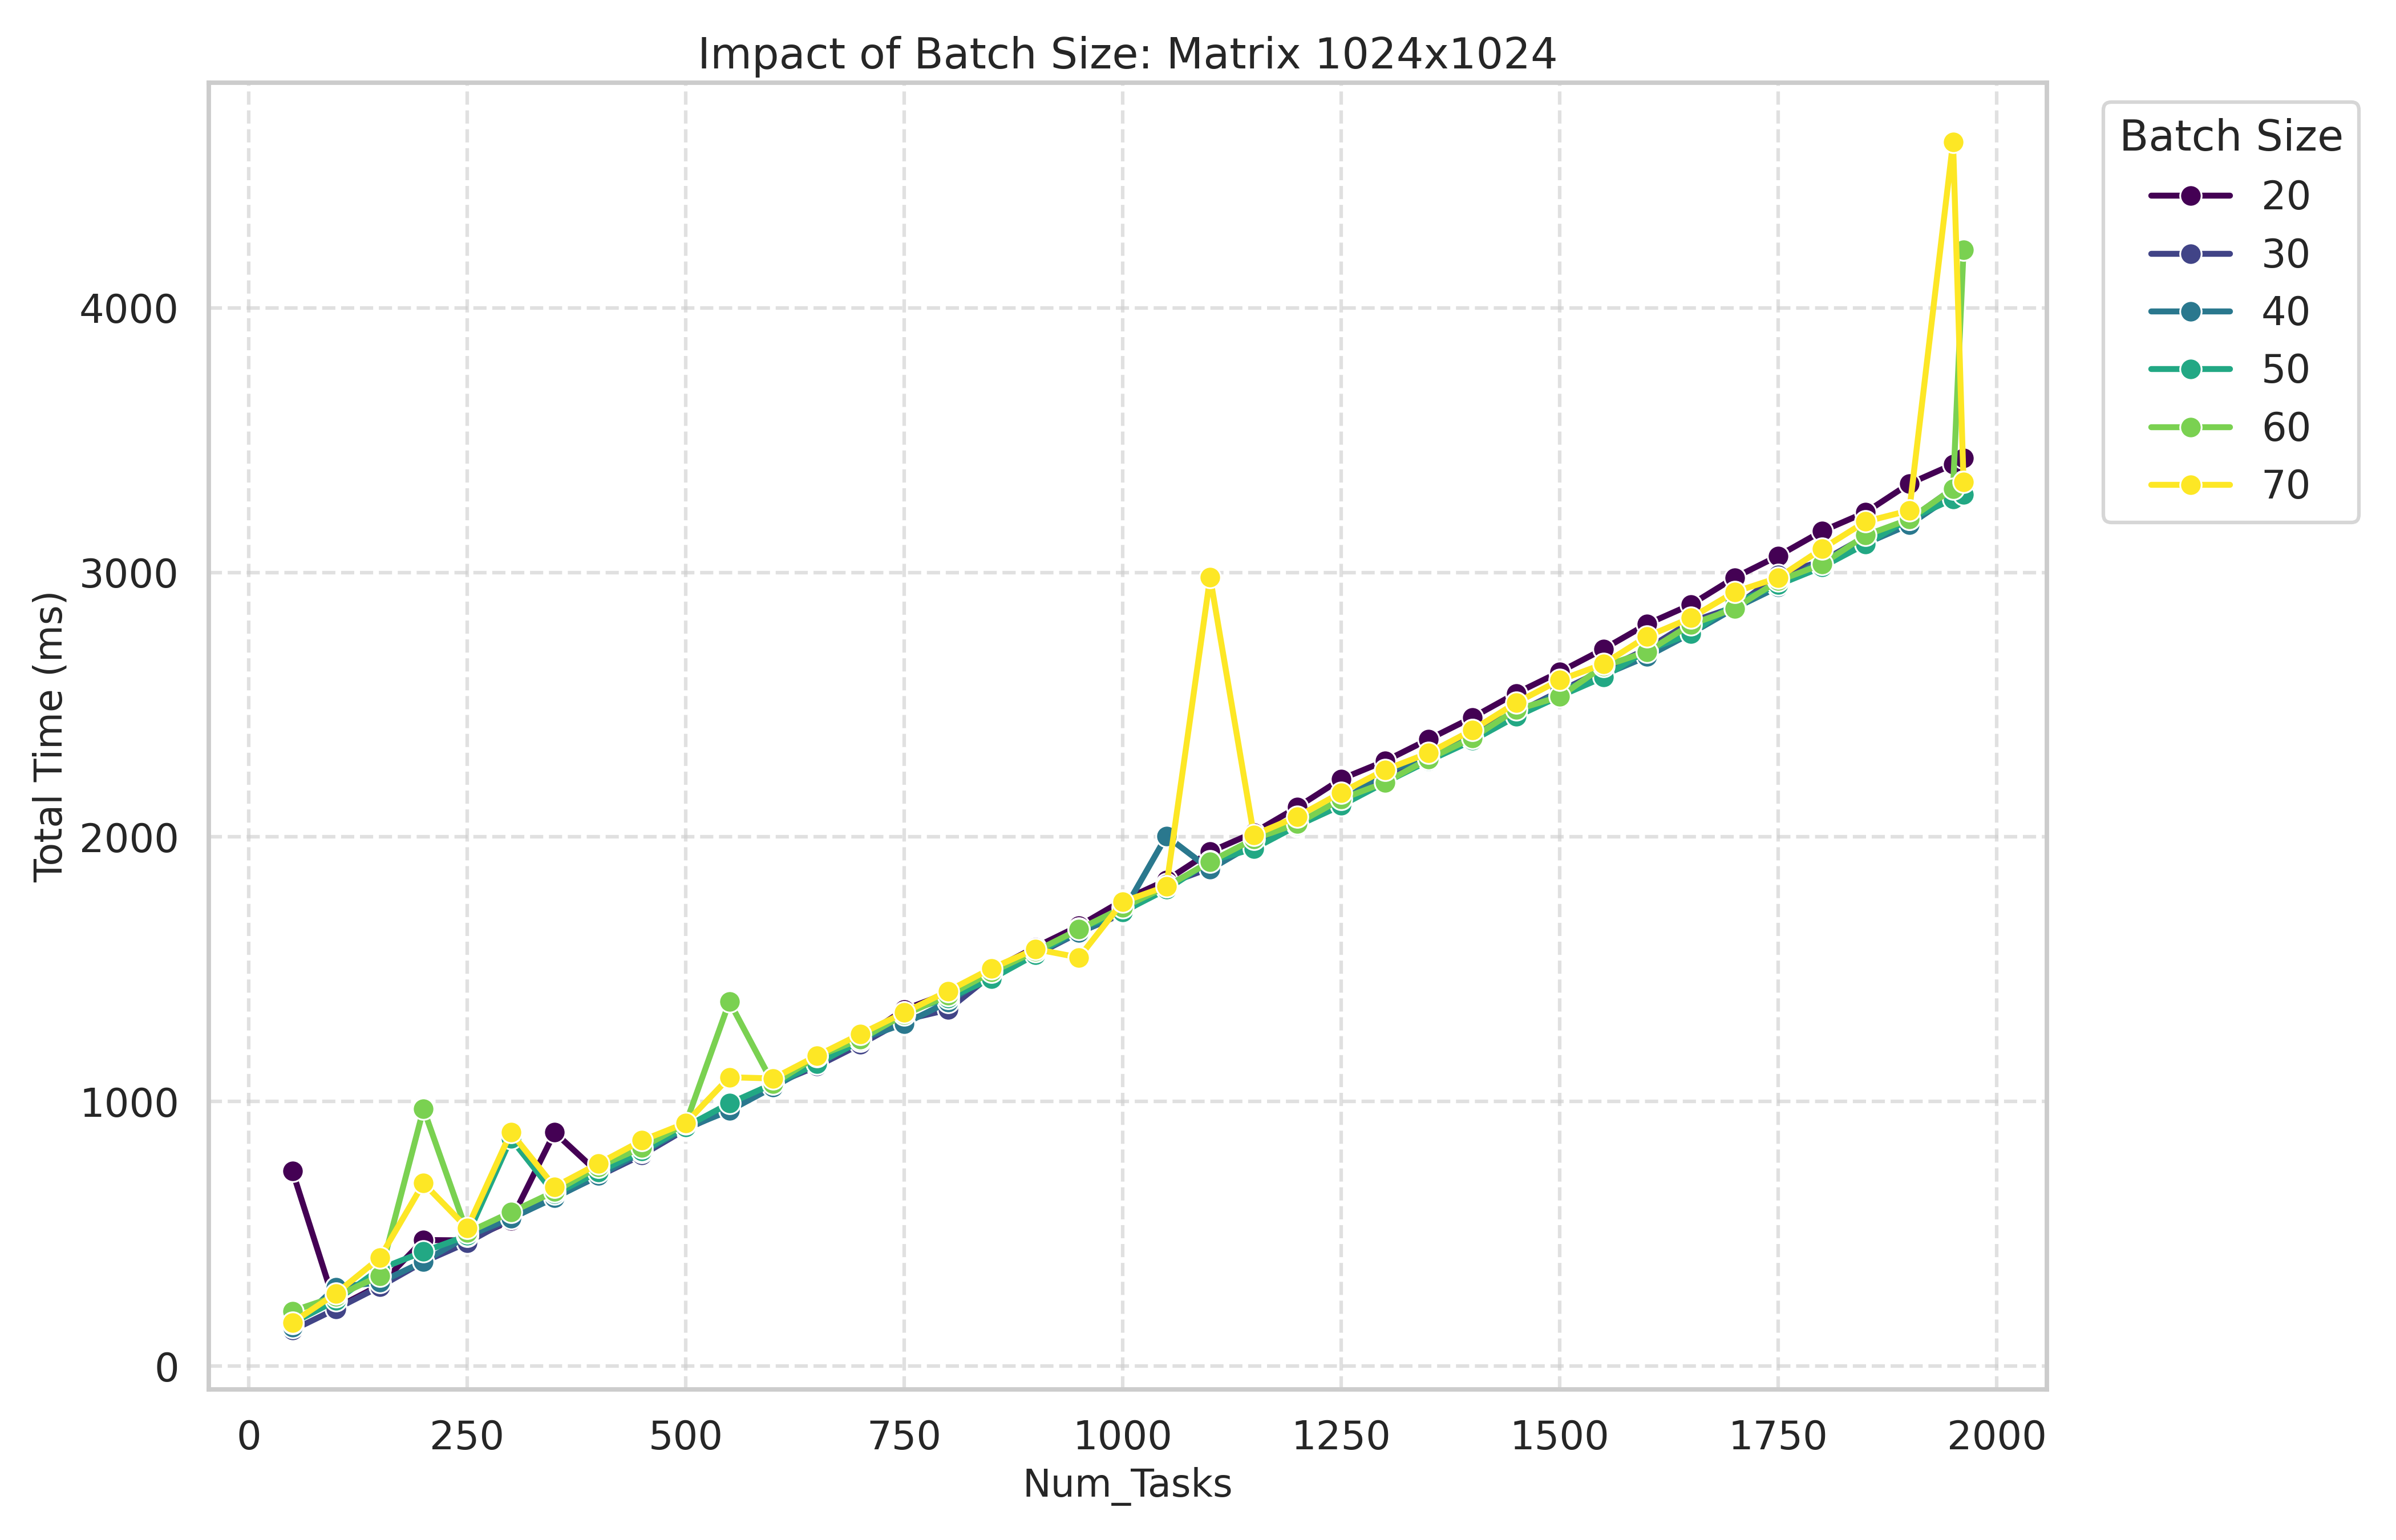
\includegraphics[scale=0.2]{images/results/analysis_batch_S1024.png} 
    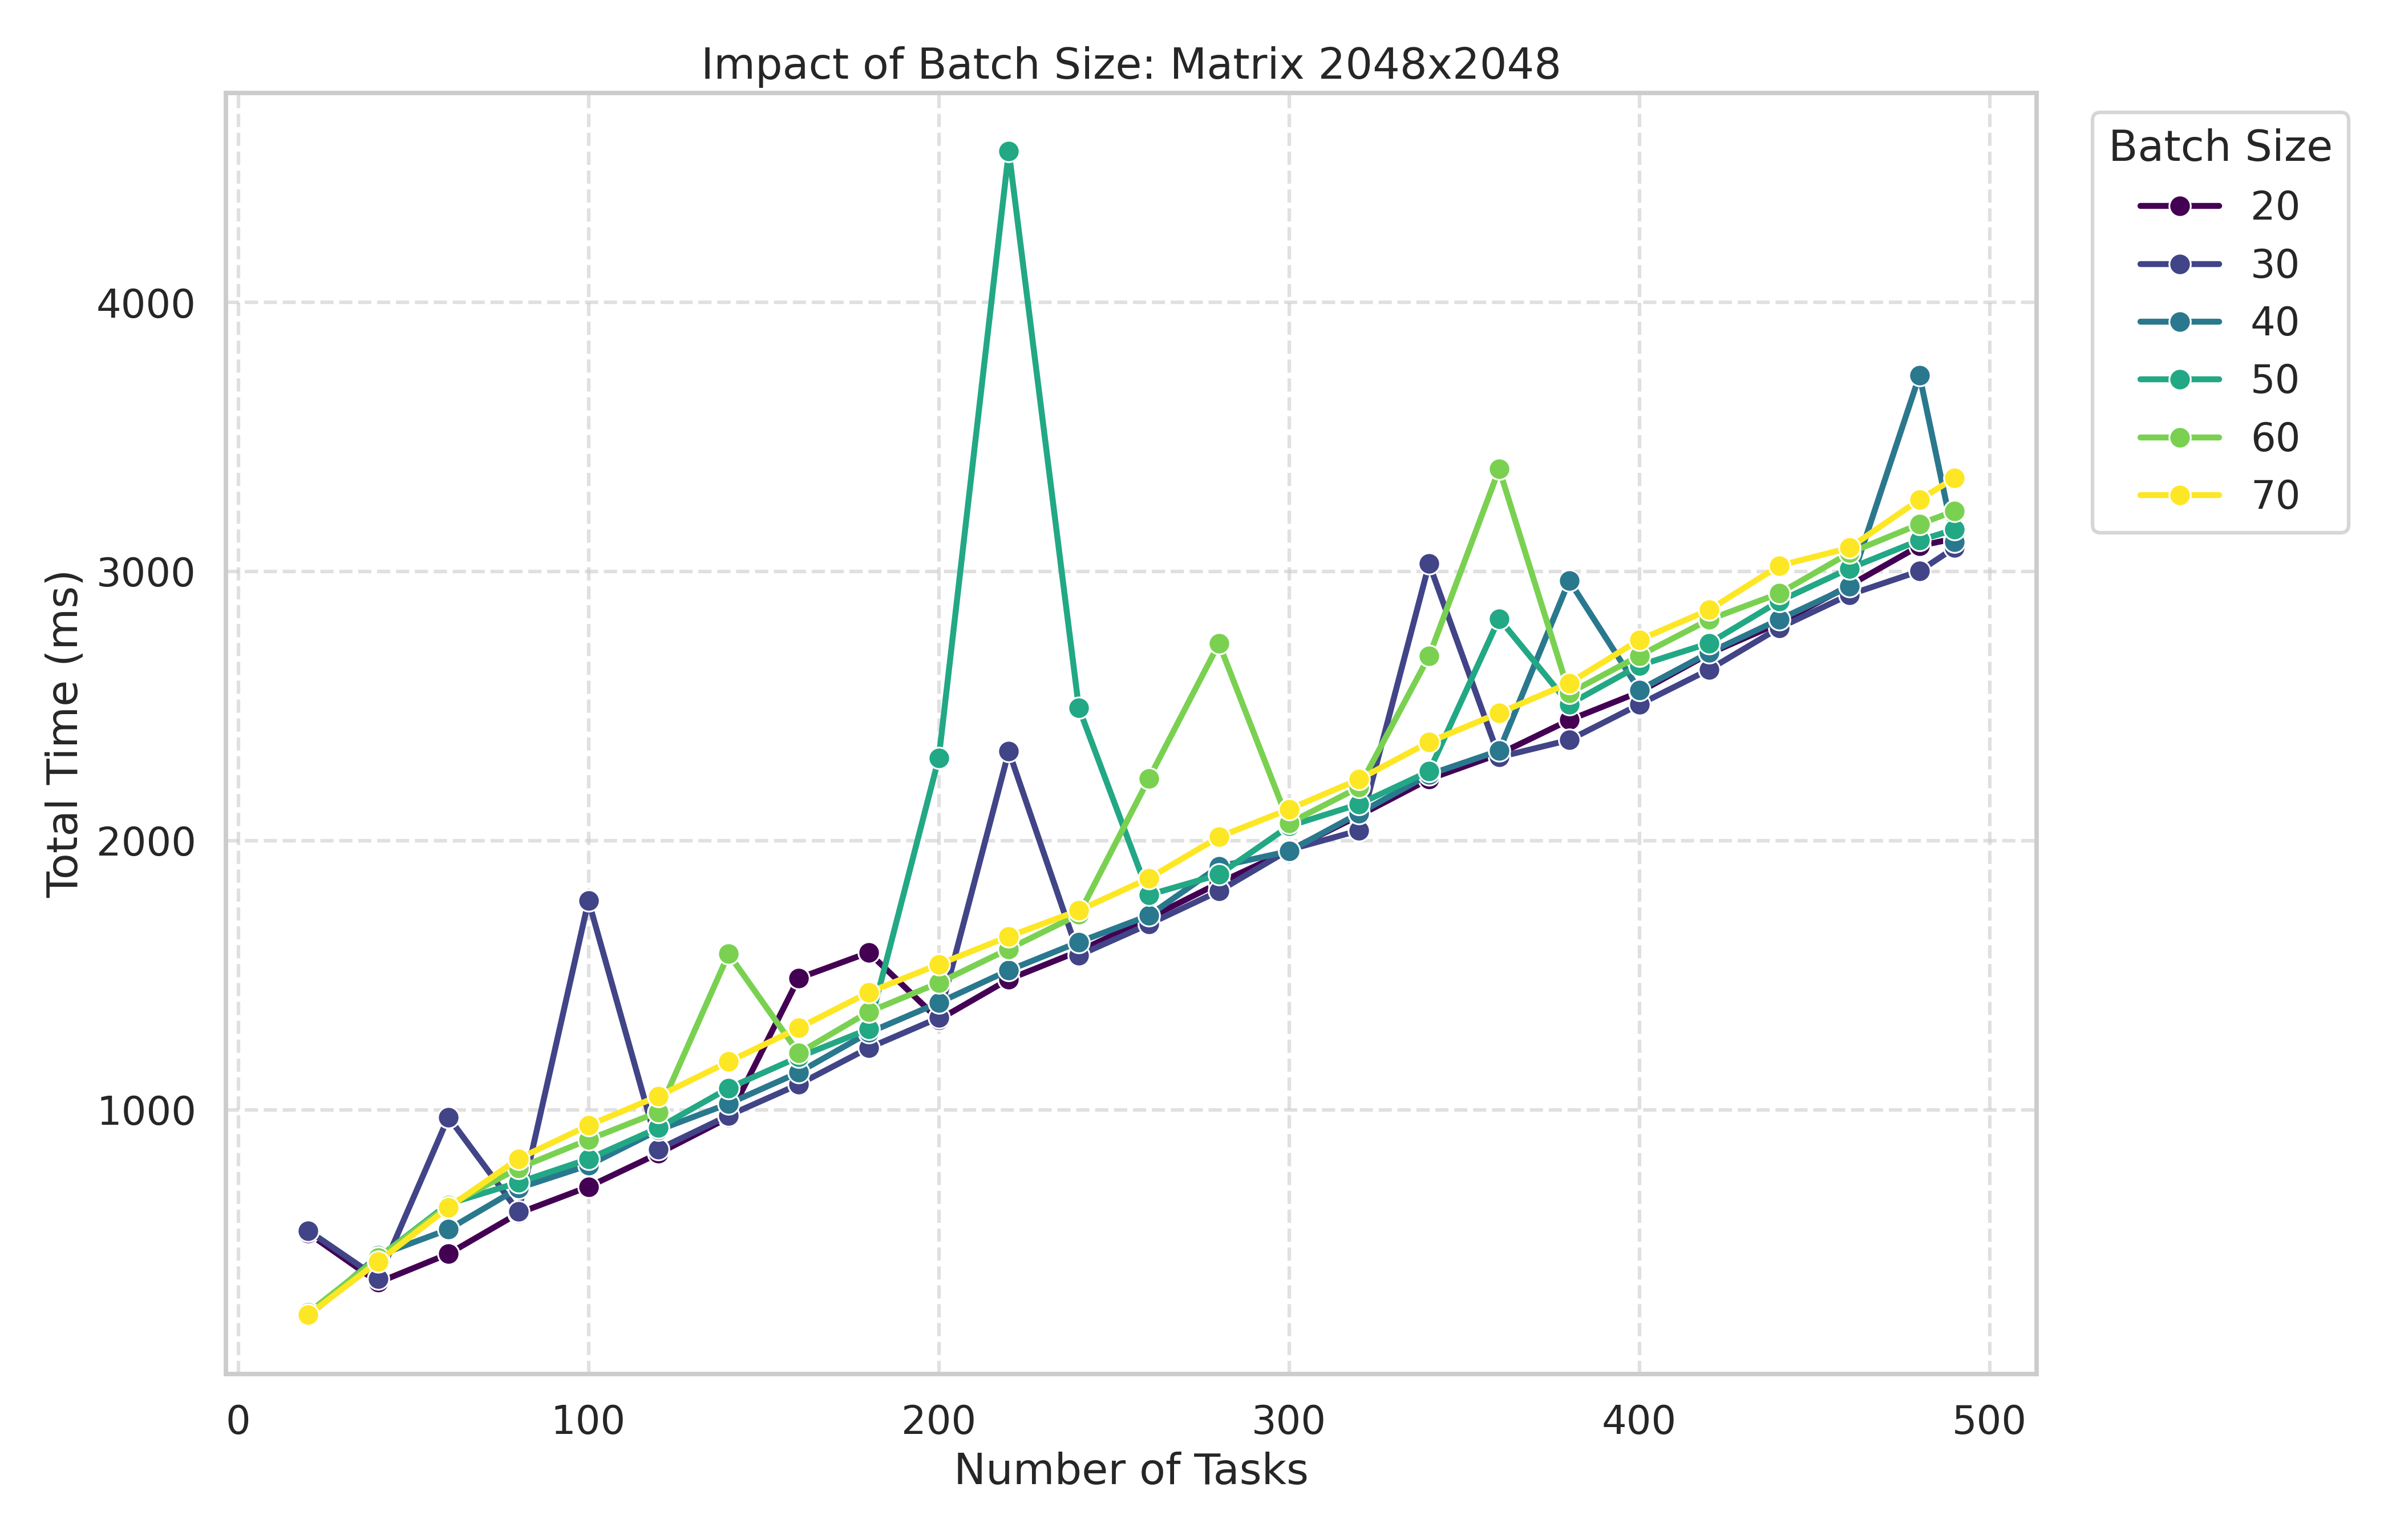
\includegraphics[scale=0.2]{images/results/analysis_batch_S2048.png} 
    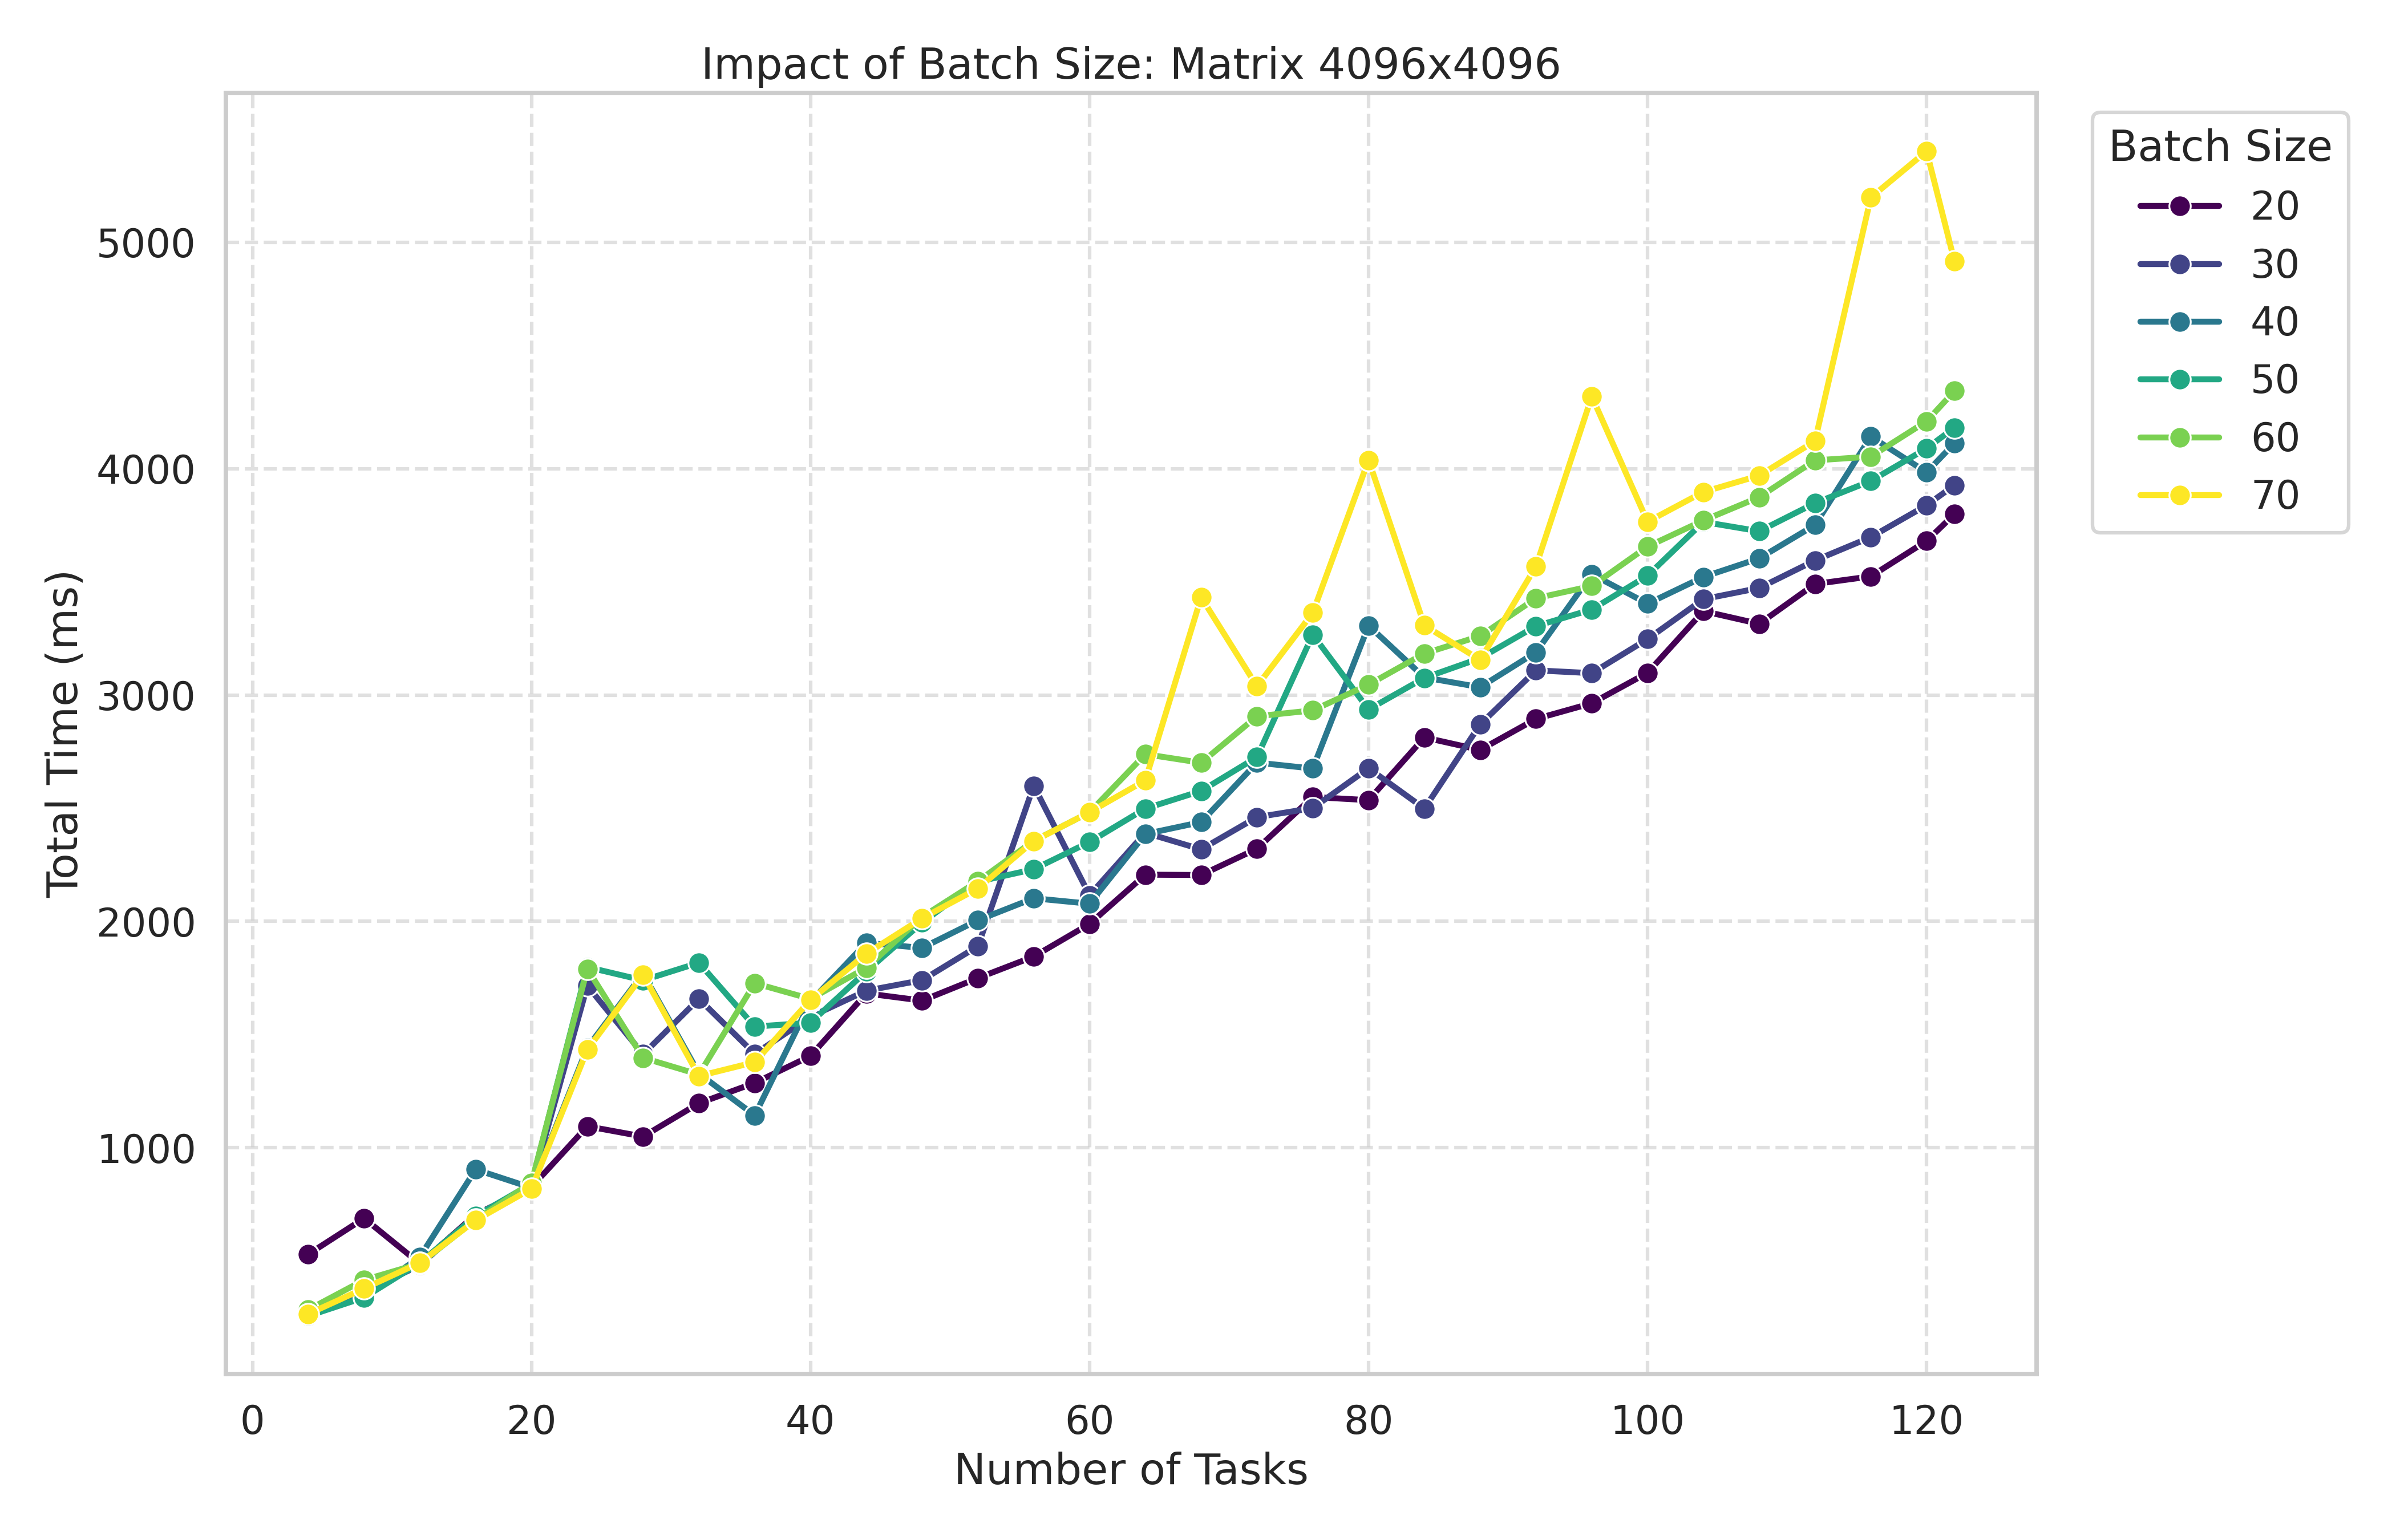
\includegraphics[scale=0.2]{images/results/analysis_batch_S4096.png} 
    \caption{Batch Size Analysis}
    \label{result1}
\end{figure}

As is evident from the graphs in Fig \ref{result1}, a relatively small batch size specifically ranging from 20 to 30 proved to be the most suitable for the selected algorithm and the dataset utilized across each workload. Conversely, it is evident that larger batch sizes frequently result in inaccurate predictions, while inevitably introducing additional overhead to the coordinator adding more time beetween the dispatch of the tasks to the workers.

\clearpage 

\section{Heterogeneous Workloads}
\subsection{Static Heterogeneous}
This test involves streams of matrices with random dimensions ( from 512 to 4096). This represents the most realistic scenario for a general-purpose system, where tasks of varying complexity arrive at the scheduler.

The results of the execution are presented in Fig. \ref{timehetero} and Fig. \ref{energyhetero}:

\begin{figure}[h!]
\centering

\includegraphics[scale=0.3]{images/results/compare_time_Hetero.png}
\caption{Time Comparison: Heterogeneous Stream}
\label{timehetero}
\end{figure}

\begin{figure}[h!]
\centering

\includegraphics[scale=0.3]{images/results/compare_energy_Hetero.png}
\caption{Energy Comparison: Heterogeneous Stream}
\label{energyhetero}
\end{figure}

As shown in Fig. \ref{timehetero}, the difference between the strategies is this case is drastic. The static hetero strategy as the red line proves to be extremely robust, consistently outperforming the single CUDA baseline as the green line. It achieves an average speedup of 1.65x (peaking at 1.85x), demonstrating how this logic achieves a consistent speedup increase while orchestrating the diverse accelerators to handle the heterogeneous workload.

In contrast, the dynamic strategy as the blue line fails to maintain consistent execution times this type of workload. With an average speedup of only 0.42x, it is significantly slower than using the discrete GPU alone. This failure is due to its greedy nature: without looking ahead, it treats a 512×512 matrix and a 4096×4096 matrix as identical tasks, and consistently fails to distribute them efficiently to achieve maximum performance.

The energy analysis in Fig. \ref{energyhetero} mirrors the performance gap already observed:
\begin{itemize}
\item \textbf{Static Strategy}: Consumes on average 112 J, achieving a -17\% energy saving compared to the average CUDA baseline (136 J).
\item \textbf{Dynamic Strategy}: Due to the extremely long execution times, the energy consumption skyrockets to an average of 805 J, with a +490\% increase over the baseline.
\end{itemize}

To better understand these results, we analyze the distribution graphs in Fig. \ref{distribhetero} and Fig. \ref{timedistrhetero}:

\begin{figure}[h!]
\centering

\includegraphics[scale=0.3]{images/results/distrib_tasks_Hetero.png}
\caption{Task Distribution: Heterogeneous Stream}
\label{distribhetero}
\end{figure}

\begin{figure}[h!]
\centering
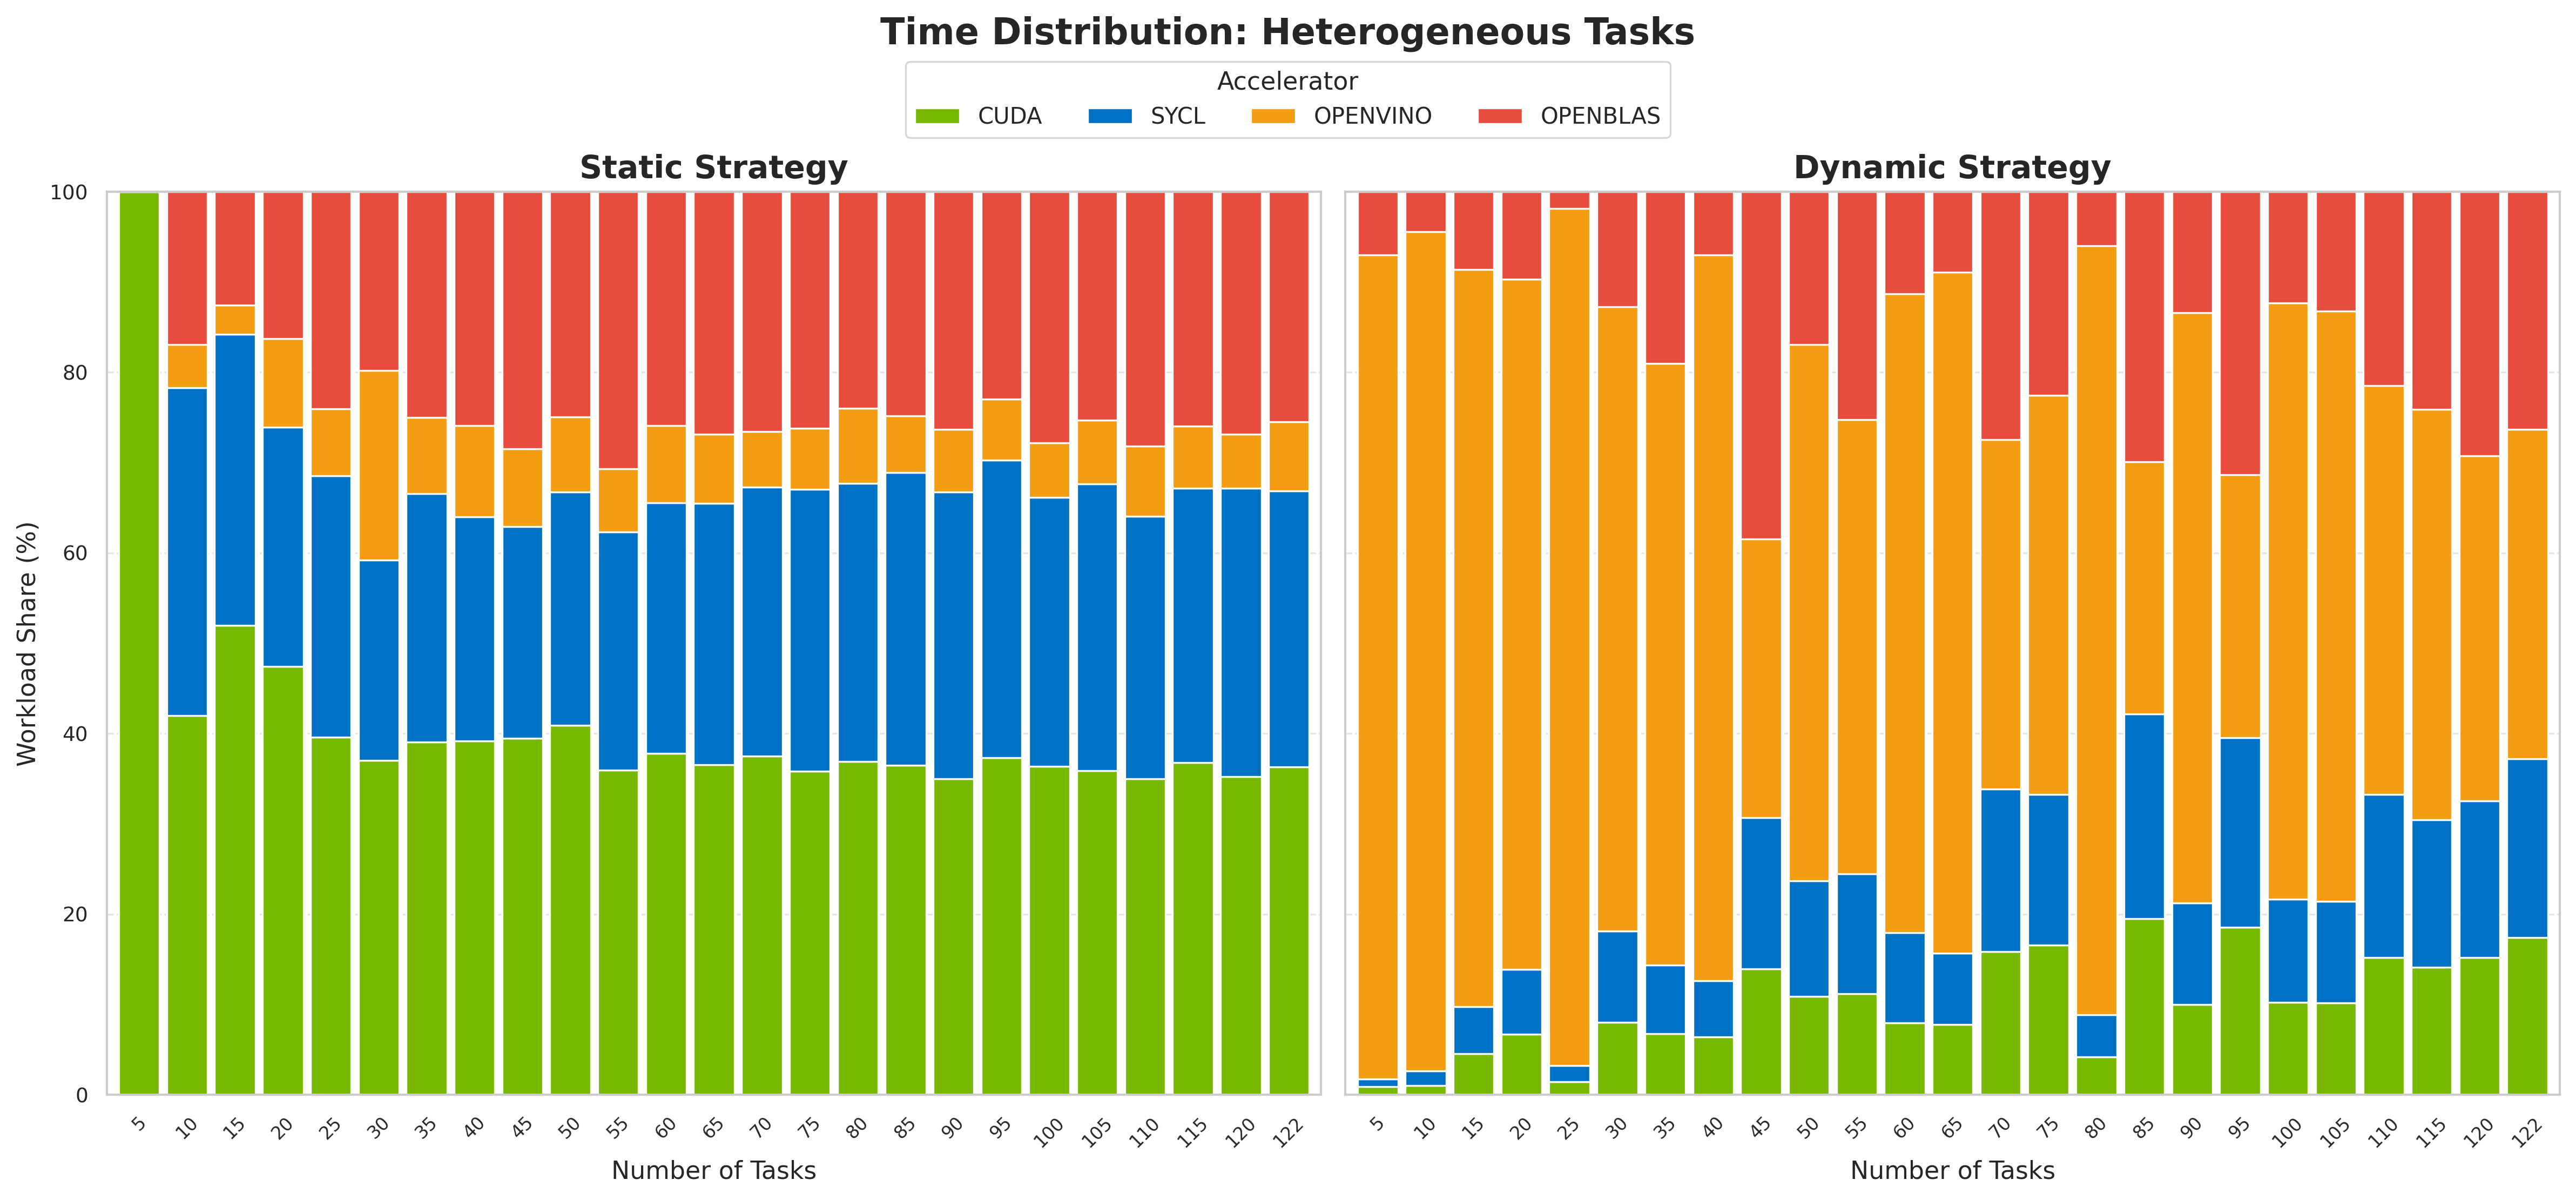
\includegraphics[scale=0.3]{images/results/distrib_Hetero.png}
\caption{Time Distribution: Heterogeneous Stream}
\label{timedistrhetero}
\end{figure}

Regarding the task distribution (see Fig. \ref{distribhetero}), the graph doesn't describe the full scenario since every task has a different weight. However, for the static strategy, we can observe that the number of tasks assigned to each accelerator remains proportional as the total number of tasks increases. This confirms that the strategy is consistent in its decision making logic.

In contrast, the dynamic strategy shows a completely chaotic behavior. Since tasks are assigned to whichever device is free, the distribution varies unpredictably. Unlike the homogeneous tests where the dynamic distribution was relatively stable with smaller tasks, here the randomness of task sizes combined with greedy scheduling leads to a random assignment that changes with every run.

As seen in the Time Distribution (Figure \ref{timedistrhetero}), the CPU and OpenVINO bars are massive. This indicates that the scheduler blindly assigned computationally heavy tasks (e.g., a 4096×4096 matrix) to slow devices simply because they were "free"" at that moment. This creates a massive bottleneck where the powerful GPU finishes its work quickly and sits idle for seconds, waiting for the CPU to finish a single large matrix.

This result conclusively proves that for heterogeneous streams of tasks, smart scheduling with performance prediction is mandatory in this kind of workloads. A simple greedy approach is insufficient and leads to severe performance degradation.

\clearpage 

\subsection{Batch Comparison}
We now present the following graph in Fig. \ref{result_hetero} to illustrate the impact of batch size on the execution times of the static logic under heterogeneous workload conditions:

\begin{figure}[h!]
    \centering
    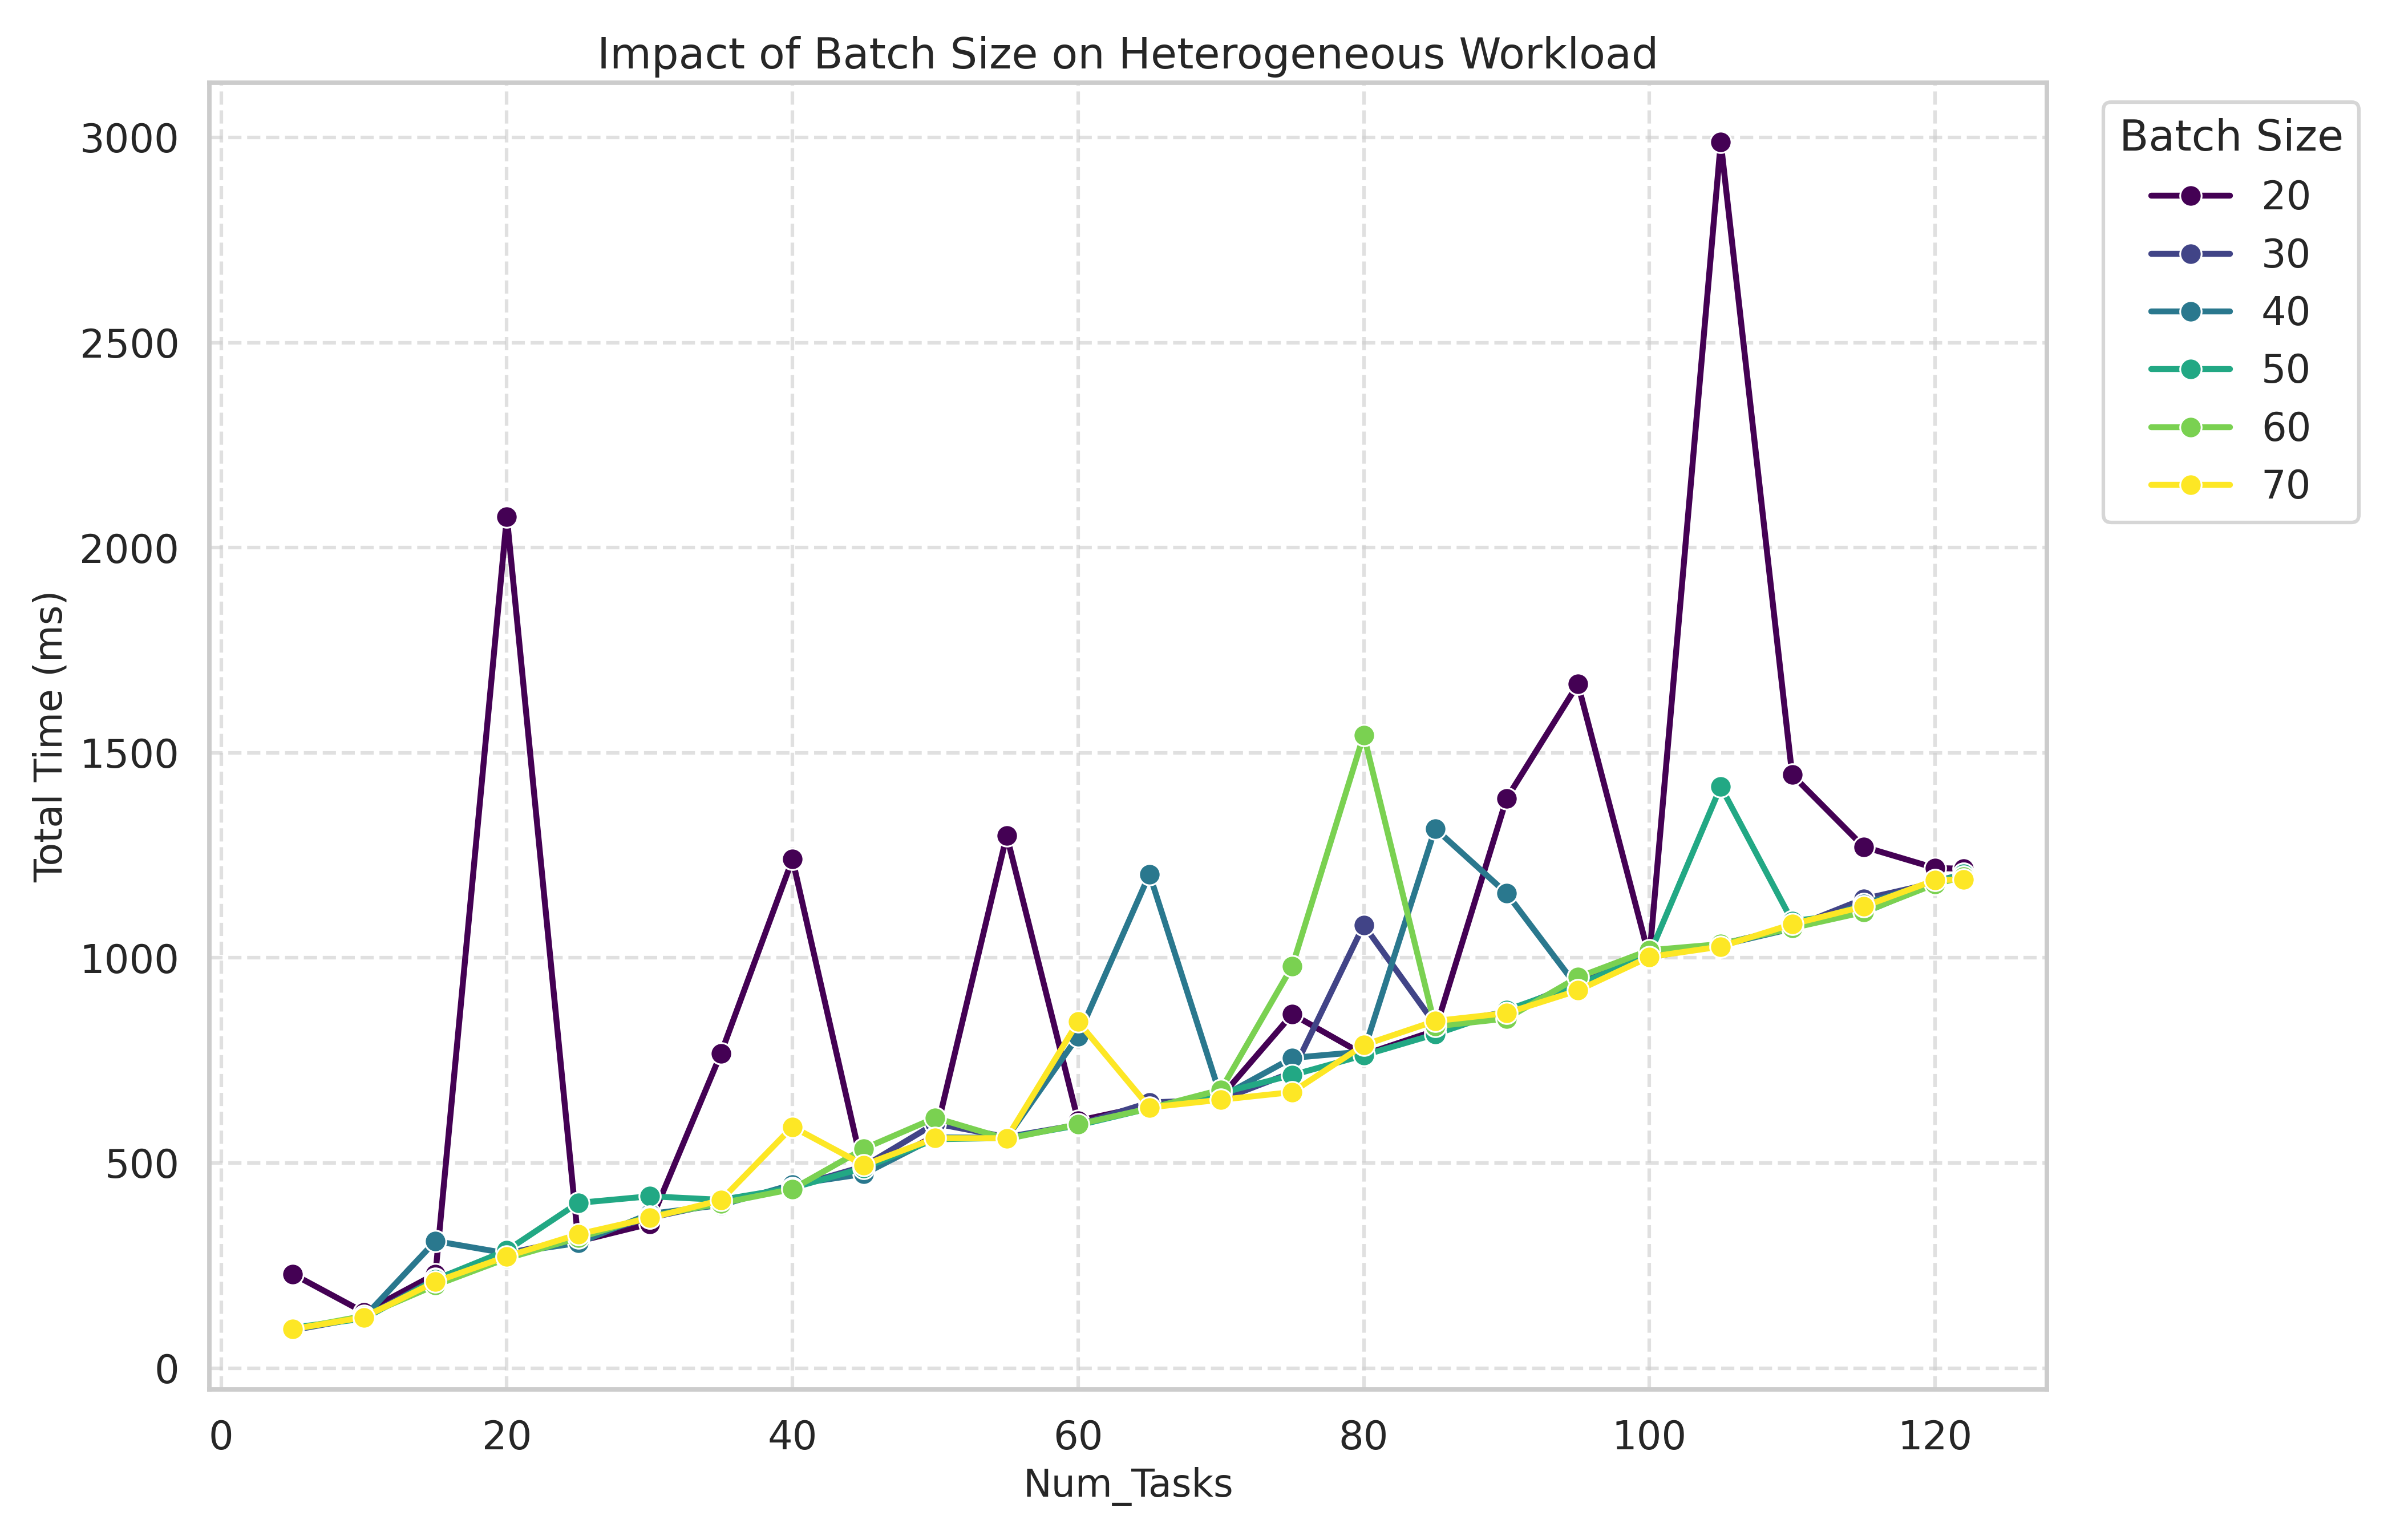
\includegraphics[scale=0.4]{images/results/analysis_batch_hetero.png} 
    \caption{Heterogeneous Batch Size}
    \label{result_hetero}
\end{figure}

As is evident from the graph in Fig \ref{result_hetero}, a relatively large batch size, specifically ranging from 60 to 70, proved to be the most suitable for the static hetero algorithm. Conversely, it is evident that smaller batch sizes (e.g. 20) frequently result in highly unstable execution times, introducing load imbalance due to the high variance of task duration. Larger batches effectively smooth out these variations, allowing the static ratios calculated within the algorithm to converge towards a more efficient distribution of the task, effectively respecting the planned times.

\subsection{Large matrix split}

This scenario involves decomposing a single very large matrix multiplication (where M grows up to 230,000 rows) into smaller sub-tasks (chunks) to fit within device memory limits and distribute the computation.

To provide a fair and meaningful baseline, a simplified version of the splitting logic was implemented. This strategy performs the same chunking operation required to handle the large matrix dimensions but dispatches all chunks exclusively to the NVIDIA GPU (the code can be seen in Appendix \ref{TODO}).

Furthermore, for this specific test case, the OpenVINO backend was excluded. Preliminary tests showed that OpenVINO's performance degrades when handling extremely "rectangular" matrices (very high M, fixed N,K), making it an unsuitable for this specific splitting workload. Our strategy therefore in this test leverages CUDA, SYCL, and OpenBLAS.

The following graphs (Fig. \ref{timelarge}) illustrate the comparison between the Hybrid Split strategy and the CUDA Only baseline:

\begin{figure}[h!]
    \centering
    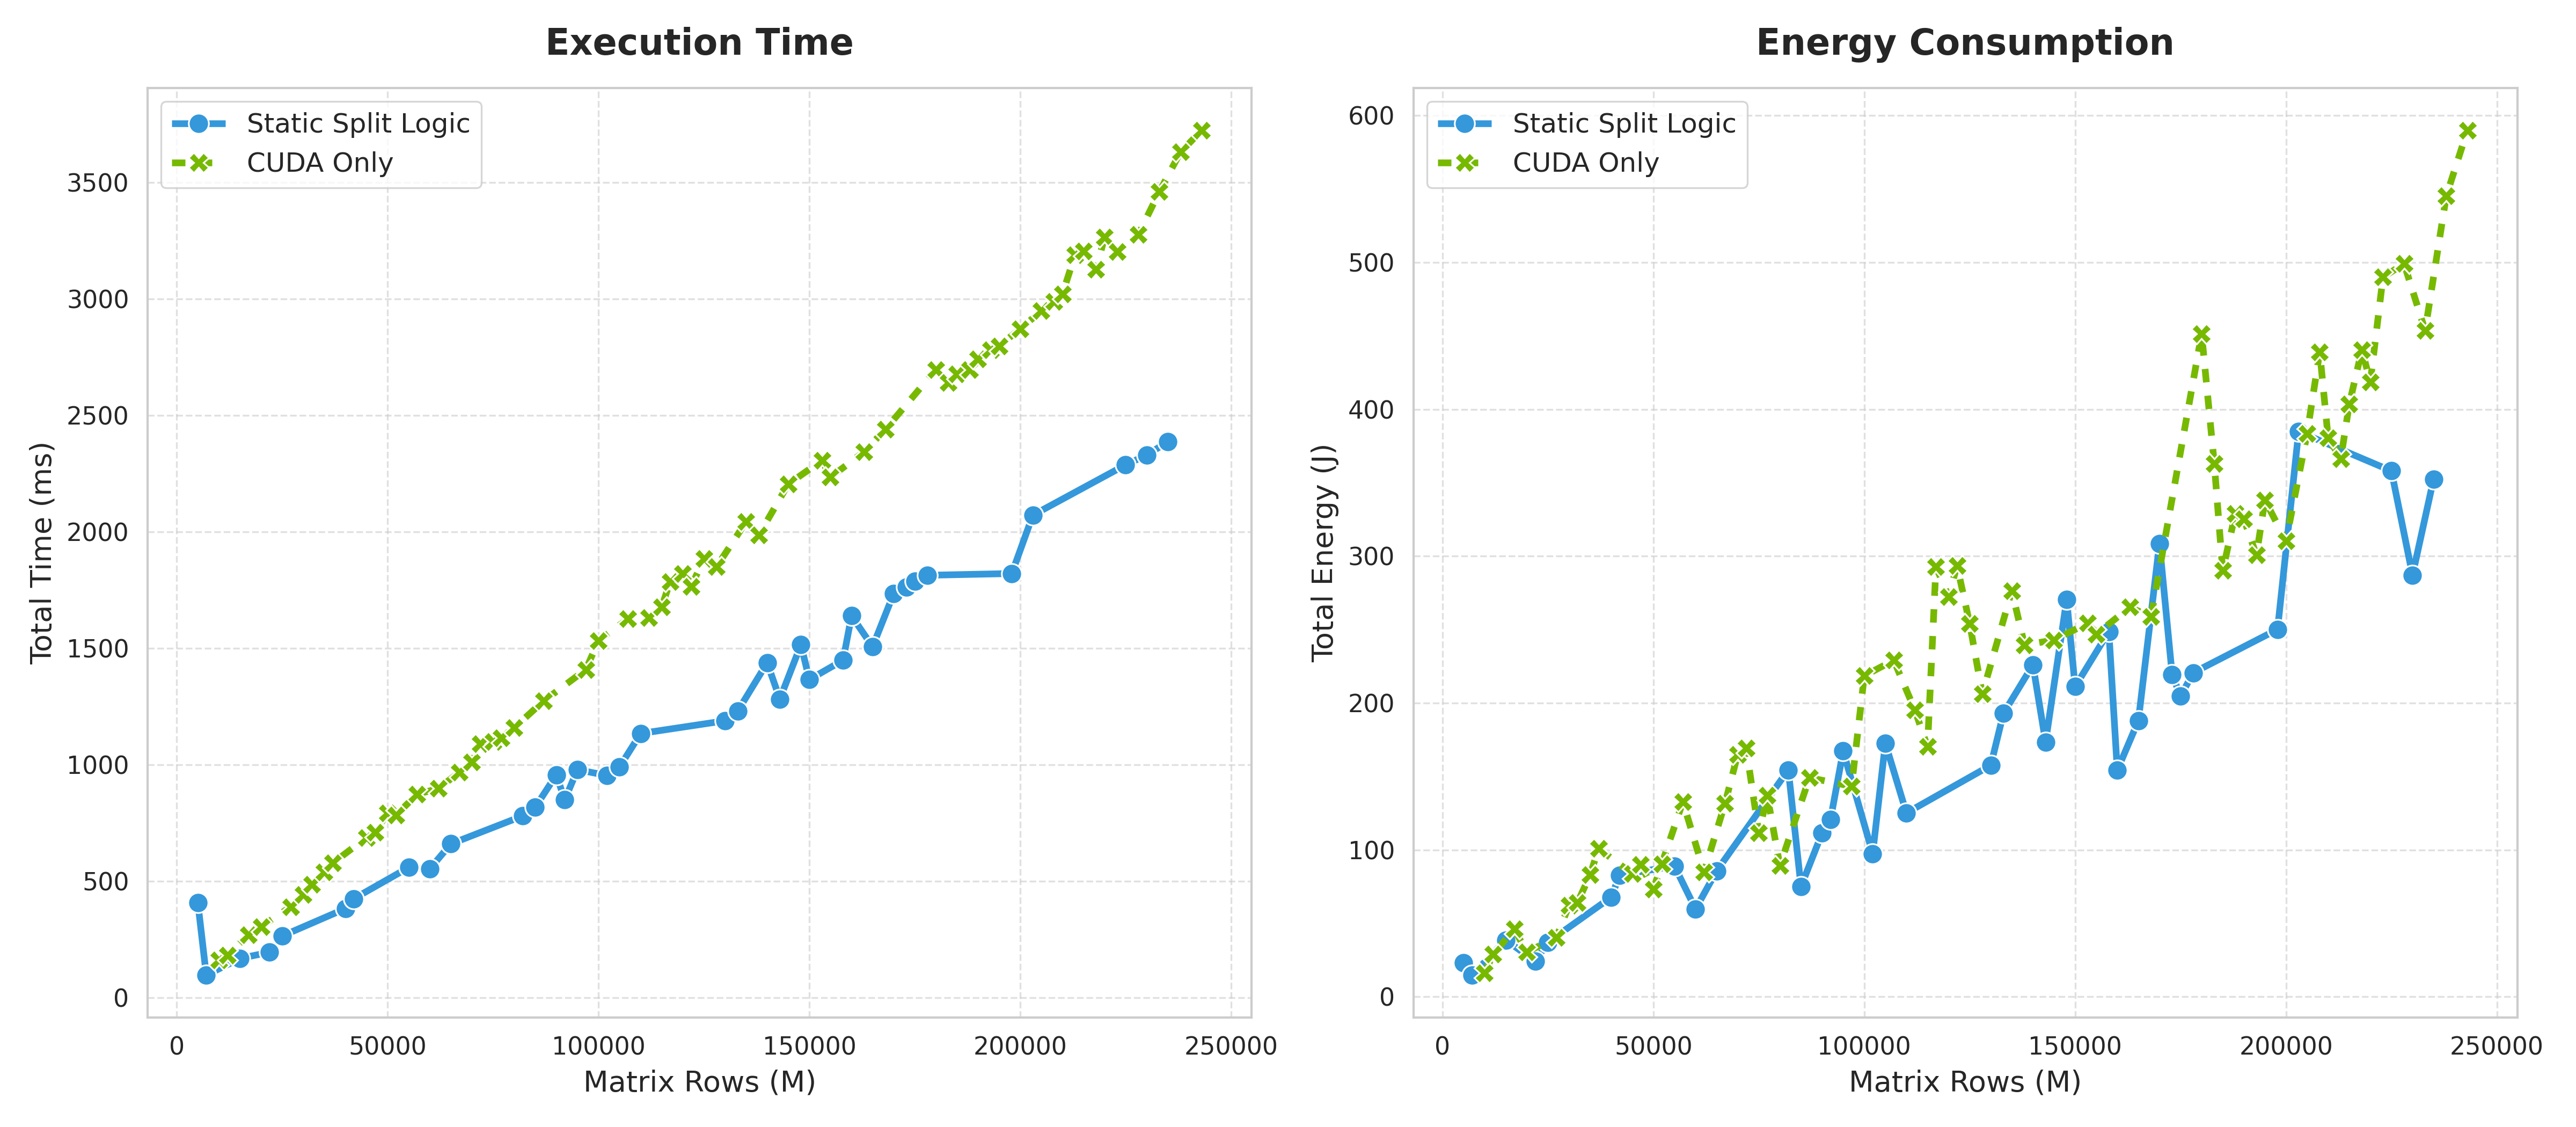
\includegraphics[scale=0.35]{images/results/large_matrix_time_energy.png} 
    \caption{Time and Task Analysis}
    \label{timelarge}
\end{figure}

The execution time comparison on Fig. \ref{timelarge} on the left clearly demonstrates the advantage of the Hybrid split approach. The split logic consistently remains below the green line (CUDA Only), indicating a lower total time to completion across the entire range of matrix sizes. The hybrid strategy achieves an 1.49x average speedup compared to using the GPU alone. In specific configurations the speedup reaches a peak of 2.46x, demonstrating that the combined throughput of the CPU and iGPU can more than double the system's performance for certain problem sizes.

Consumptions wise, the Hybrid strategy also demonstrated superior energy efficiency in some cases (see Fig. \ref{timelarge} on the right): on average, the large static split approach reduced energy consumption by 21\% compared to the CUDA baseline. Furthermore over the entire benchmark, the hybrid strategy consumed 38 J less on average than the 52 J required by the CUDA only execution. This result highlights that finishing the task faster, even by powering up the CPU and iGPU, is often more energy efficient than keeping the discrete GPU active for a longer duration.

\clearpage

\begin{figure}[h!]
    \centering
    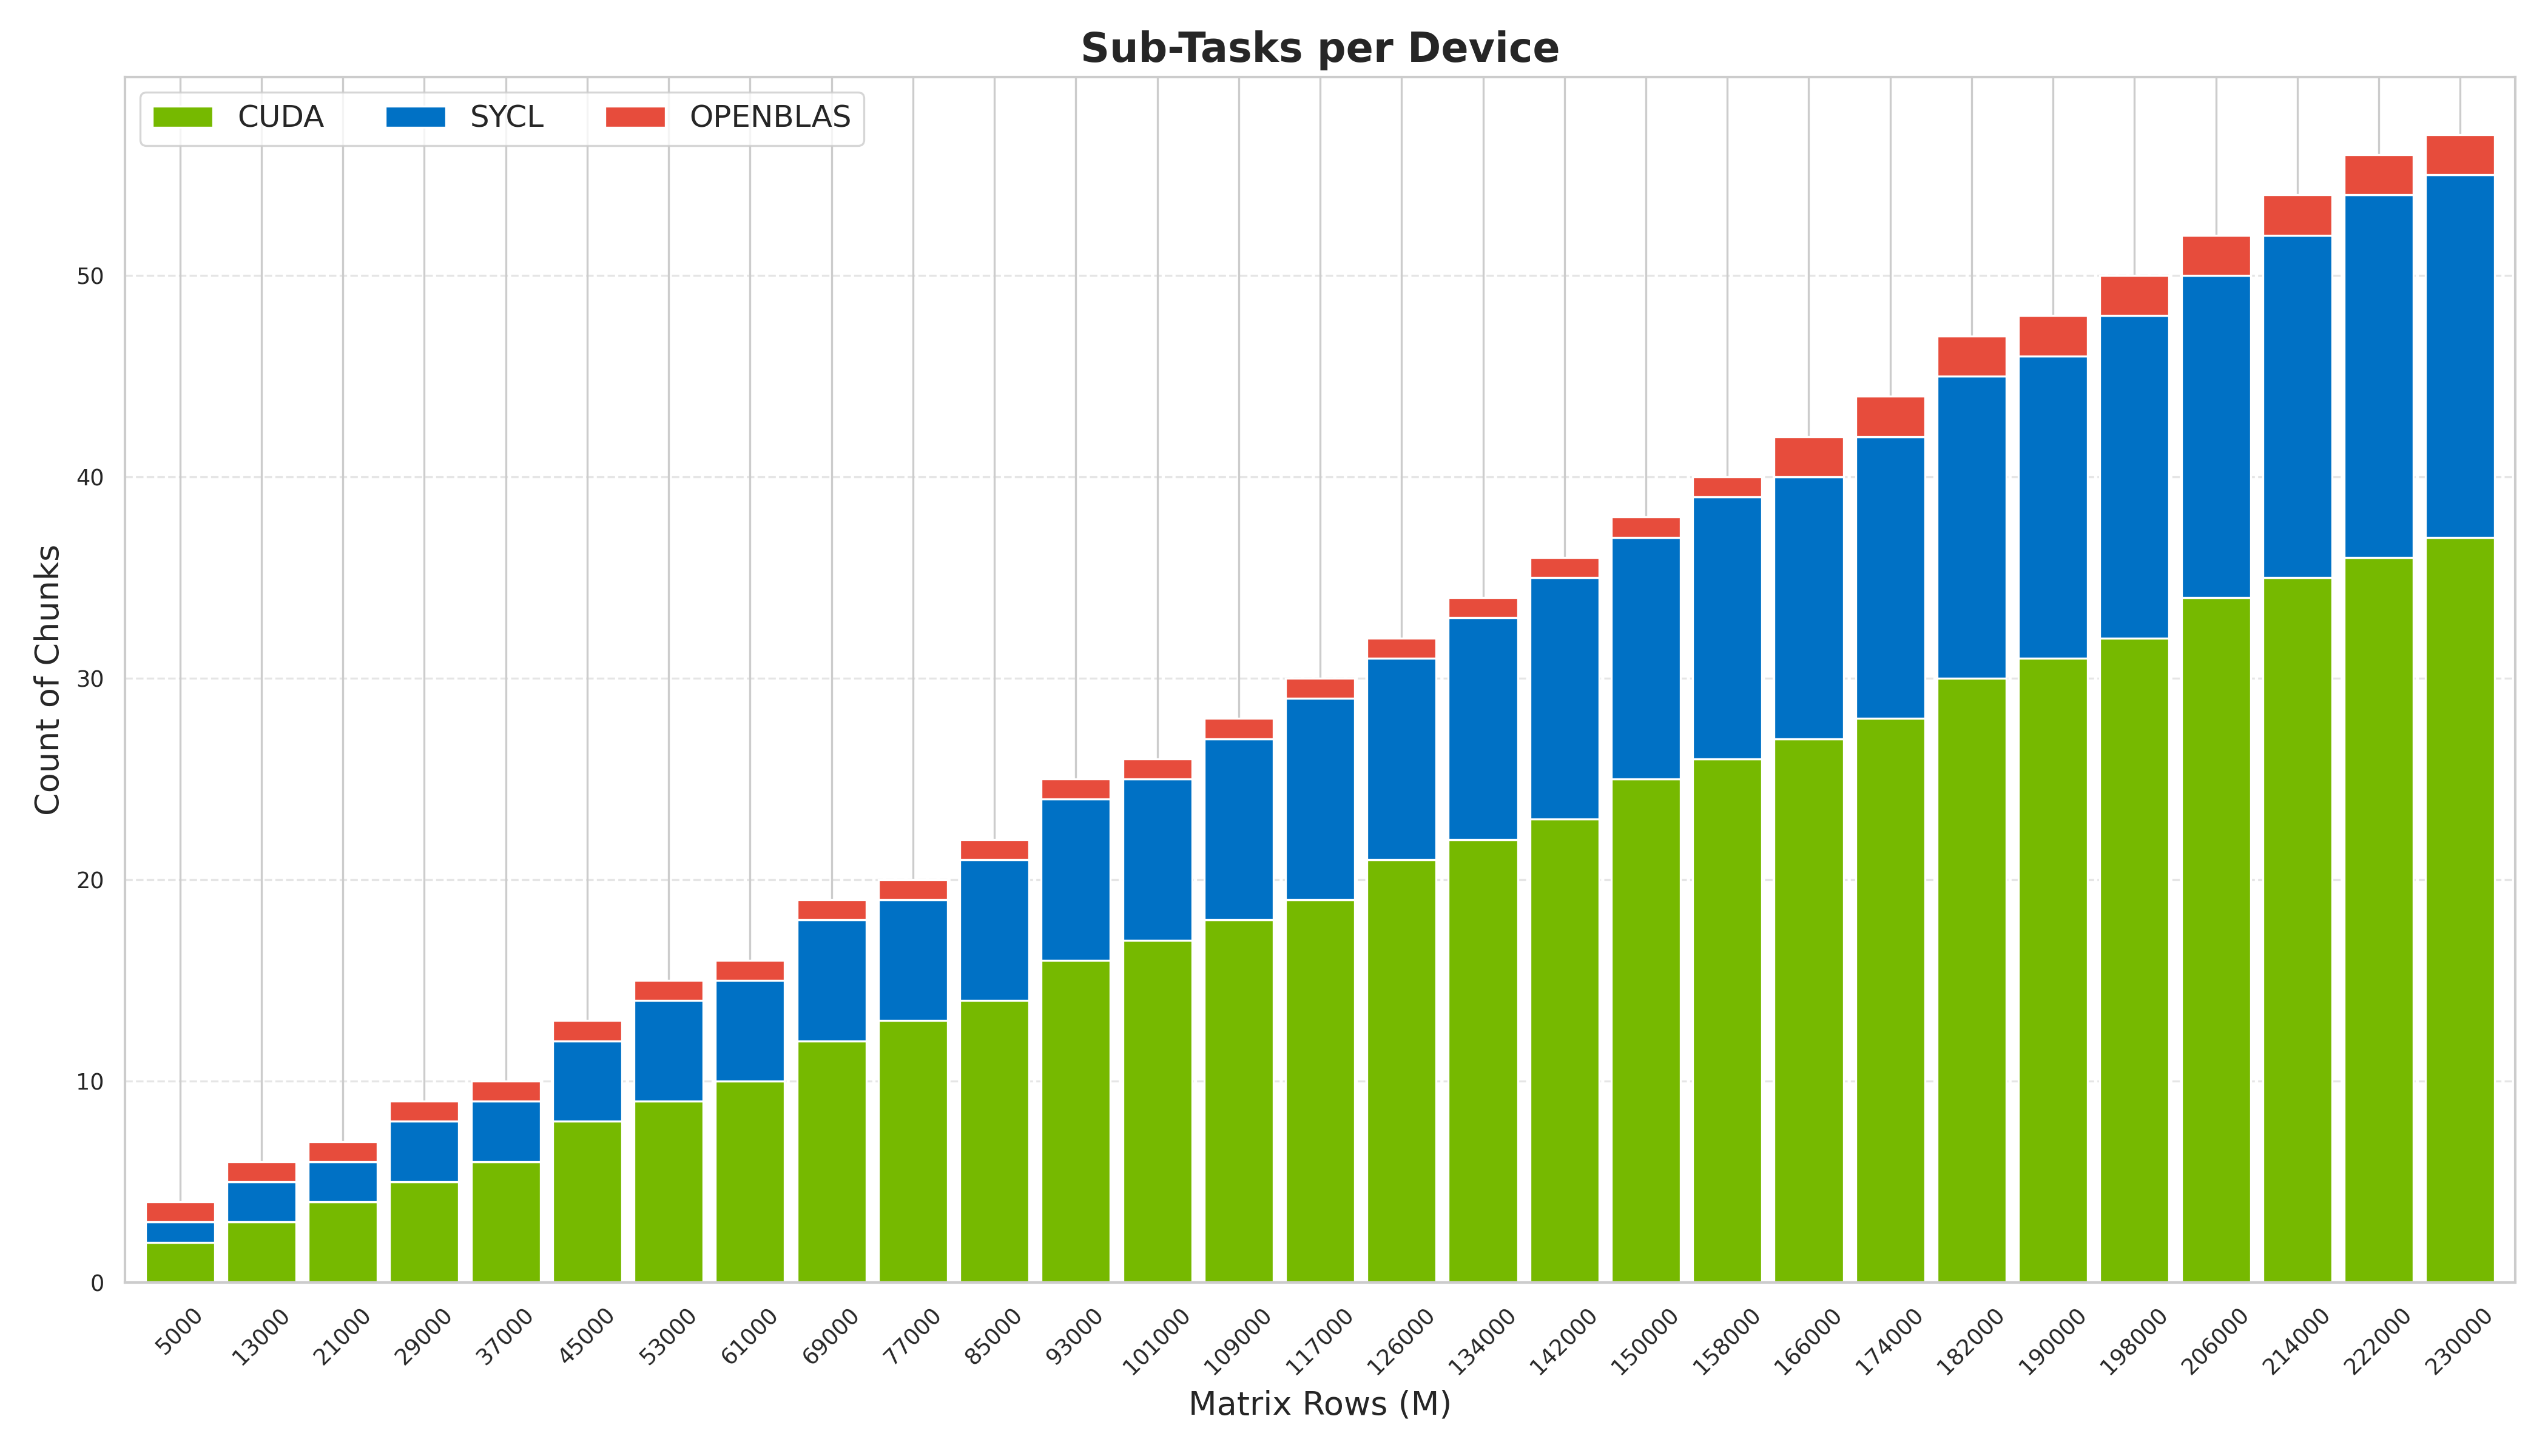
\includegraphics[scale=0.4]{images/results/large_matrix_chunks.png} 
    \caption{Chunk Distribution Analysis}
    \label{chunklarge}
\end{figure}

The load balancing graph on Fig. \ref{chunklarge} provides insight into how the work was distributed. As expected, the powerful CUDA GPU handles the majority of the chunks (approximately 50\% or 60\% of the workload). The remaining of the work is successfully offloaded to the iGPU and CPU backends. This is the direct cause of the observed speedup: by keeping all accelerators active, the system completes the massive calculation faster than the single GPU could.
